\chapter{Fundamentação teórica}\label{cap_trabalho_academico}

\section{Infraestrutura Urbana}
A infraestrutura urbana compreende o conjunto de serviços e estruturas essenciais ao funcionamento das cidades, incluindo saneamento básico, iluminação pública, pavimentação de vias e condições adequadas de calçadas. A gestão desses elementos é responsabilidade dos órgãos administrativos, sendo fundamental para garantir qualidade de vida, mobilidade e segurança à população.

Em diversos municípios, observam-se deficiências relacionadas à infraestrutura urbana, como a presença de buracos em vias e calçadas, falhas na sinalização, focos de água parada e problemas na iluminação pública. Em muitos casos, essas situações persistem por longos períodos, evidenciando limitações nos processos de identificação, registro e resolução dessas ocorrências.

A ausência de canais estruturados de comunicação entre a população e o poder público contribui para o agravamento desses problemas, dificultando o acompanhamento das demandas e a transparência das ações realizadas. Nesse contexto, o uso de tecnologias digitais surge como uma alternativa para melhorar o registro, o monitoramento e a gestão de problemas urbanos, possibilitando maior eficiência na administração pública.


\section{CIDADES INTELIGENTES}
O conceito de Cidades Inteligentes tem ganhado destaque na sociedade contemporânea. De acordo com uma publicação da PUC-RS: 
\begin{citacao}
    Cidades inteligentes, ou \textit{smart cities}, são cidades que conseguem alinhar o desenvolvimento tecnológico com o progresso social e ambiental, por meio de inovações digitais e disruptivas. O objetivo dessas estratégias de desenvolvimento urbano é proporcionar aos cidadãos uma melhor qualidade de vida. \cite{puc_cidades_inteligentes}
\end{citacao}

O uso de tecnologias de coleta de dados em tempo real são fundamentais para as iniciativas de cidade inteligente. Os dados obtidos possibilitam que os governos locais tenham um melhor planejamento e realizem ações de maneira mais pontual e eficaz. Dentre os benefícios que a implementação do conceito de cidades inteligentes estão: gerenciamento de resíduos, melhorias no transporte público, melhorias no planejamento municipal entre outros. \cite{cidadeintelignte_ibm}

Tal conceito alinha-se com a proposta de um aplicativo em que a população consegue registrar os problemas de infraestrutura que enfrentam no seu dia-a-dia, sendo possível usar a tecnologia para coleta de dados e posteriormente, uma análise das melhores ações a serem tomadas pelas autoridades competentes.

As cidades inteligentes são soluções para decisões ruins de design das cidades do século passado. Congestionamento, alertas globais, declínio da saúde, todos esses problemas serão poderão ser computados. O que hoje são controles manuais, serão realizados por sensores, softwares e redes de computadores, proporcionando eficiência, predições e diminuições de riscos. \cite{townsend_smartcities}.

\section{TECNOLOGIAS NA GESTÃO URBANA}
O uso de tecnologias de informação e comunicação vem apresentando um alto crescimento em diversos países. A utilização de \textit{softwares}, sensores, \textit{websites} para registro, acompanhamento e monitoramento de situações urbanas como trânsito, segurança, emergências vêm sendo comum em municípios do Brasil. 

De acordo com uma pesquisa realizada em 2019 pelo CETIC.br, cerca de 21\% das prefeituras pesquisadas haviam um centro de operações dedicado a monitorar situações como trânsito, segurança ou emergência\cite{nicbr_cidades_inteligentes_2020}. Entre as prefeituras com centros de operações funcionando, 86\% declararam monitorar a segurança pública, seguido de trânsito (73\%), patrimônio ou prédios públicos (71\%); e situações de emergências ou desastres (54\%). 

A oferta de serviços públicos digitais, também popularmente conhecidos como e-serviços, constitui um alto nível de maturidade tecnológica na gestão pública. Esses serviços permitem que os cidadãos solicitem serviços e acessem informações públicas sem a necessidade de se deslocar fisicamente até a prefeitura ou outros órgãos administrativos, melhorando a eficiência e comodidade dos cidadãos.

No entanto, estudos indicam que a disponibilização de e-serviços ainda é limitada em grande parte dos municípios brasileiros. Enquanto capitais apresentam mediana de pontuação mais elevada, municípios de menor porte frequentemente não atingem níveis satisfatórios de oferta desses serviços, evidenciando desigualdades regionais e estruturais\cite{nicbr_cidades_inteligentes_2020}. Além disso, observa-se que a existência de infraestrutura tecnológica não garante, necessariamente, a efetiva prestação de serviços digitais à população, o que reforça a necessidade de soluções que priorizem as demandas reais dos cidadãos.


\begin{figure}[htb]
    \centering
    \caption{\label{fig1_mediana}Medianas de Pontuação para E-serviços Públicos, por região}
    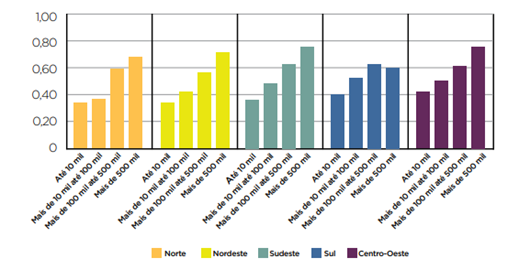
\includegraphics[scale=1.0]{images/figuras/fig1_mediana_eservicos.png}
    \fonte{\citeonline{nicbr_cidades_inteligentes_2020}}
\end{figure}

De acordo com uma pesquisa realizada por meio da PNAD Contínua\cite{ibge_celular}, cerca de 167,5 milhões de brasileiros com 10 anos ou mais de idade já possuíam um telefone celular para uso pessoal. Isto corresponde a 88,9\% da população naquela faixa etária. 

\section{PARTICIPAÇÃO CIDADÃ}

A participação cidadã compreende a participação da população nos processos de formulação, execução e avaliação de políticas públicas, constituindo um elemento essencial para garantia de direitos sociais \cite{participacao_cidade_parlamento}. Nesse contexto, é essencial que a participação cidadã englobe a população como um todo na elaboração de políticas públicas, permitindo que as tomadas de decisões governamentais atinjam as demandas de diversos segmentos sociais, incluindo os segmentos populacionais marginalizados e os com pensamentos divergentes. \cite{pintaudi_participacao_cidada}

No âmbito urbano, os problemas de infraestrutura e saneamento são aspectos que afetam diversos pontos da sociedade, principalmente em bairros mais periféricos e afastados dos principais centros comerciais do município. 

Com esse enfoque, Jacobs(\citeyear{jacobs_american_cities}) destaca que "as cidades têm a capacidade de fornecer algo para todos, apenas porque, e apenas quando, são criadas por todos”, evidenciando a participação coletiva e democrática na elaboração de soluções e gestão dos espaços urbanos. 

\section{GEOLOCALIZAÇÃO}
Conforme já visto anteriormente, o conceito de cidades inteligentes vem crescendo em várias metrópoles mundiais, por meio do uso de ferramentas de coleta de dados aliadas à gestão pública, com o intuito de melhorar a qualidade de vida dos cidadãos. Dentre as ferramentas destaca-se a geolocalização.

A geolocalização ou georreferenciação trata-se de uma tecnologia que permite determinar a localização geográfica de um objeto ou pessoa com base em coordenadas ou permite utilizar a localização dos dispositivos para fins de coleta de dados, rastreamento, mapeamento, entre outras aplicações. A Geopixel, empresa reconhecida nacionalmente pelo fornecimento de soluções de geointeligência para prefeituras, define a geolocalização como: 

\begin{citacao}
    A geolocalização é a tecnologia que permite determinar a localização exata de um objeto, pessoa ou imóvel na superfície terrestre, usando coordenadas geográficas (latitude e longitude). Pode ser feita via GPS, redes móveis, satélites, endereços IP, entre outras fontes. 
    \cite{geopixel}
\end{citacao}

De acordo com Kurkdjian e Pereira (2006 apud \citeauthoronline{silva2013geotecnologias}, 2013, p. 9-10), ferramentas de geolocalização já são ativamente utilizadas em outros contextos como estudos da expansão urbana, dinâmica da utilização do solo seja residencial, comercial, de serviços ou industrial.

\section{PROBLEMAS ENFRENTADOS NO MUNÍCIPIO DE ITU}
Com base nas respostas de 303 cidadãos ituanos para a Pesquisa Prioridades, uma pesquisa realizada em 2025 sobre os 3 principais problemas que a cidade enfrenta, as respostas coletadas apontaram que a saúde seria o principal problema enfrentado com 70\% das respostas, água e esgoto estando como segundo principal problema com 57\% das respostas e em terceiro lugar asfalto/buracos com 39\% das respostas.  \cite{portalopiniao}

\begin{grafico}[htb]
    \centering
    \caption{Principais prioridades requisitadas pelos munícipes de Itu}
    \label{graf:prioridades_itu}
    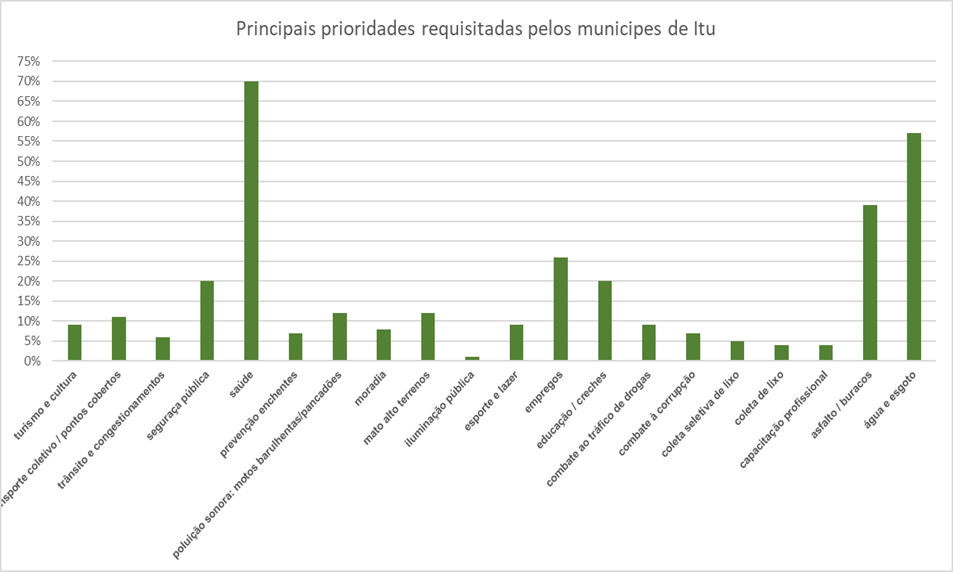
\includegraphics[width=\textwidth]{images/graficos/graf1_prioridades.png}
    \fonte{Adaptado de \citeonline{portalopiniao}}
\end{grafico}

Somente no período de 4 meses de 2025, entre o dia 1º de janeiro até o dia 24 de abril, foram registrados cerca de 4.350 casos confirmados de dengue na cidade de Itu, sendo a principal distribuição de casos para pessoas entre 40 a 59 anos, com 1308 casos confirmados. Como é de conhecimento do leitor, uma das principais maneiras de proliferação do mosquito transmissor da dengue é através de focos de água parada, que, em muitas das vezes, concentram-se em áreas de vias públicas e/ou locais abandonados que necessitam de resolução da prefeitura. \cite{arboviroses}

\begin{grafico}[htb]
    \centering
    \caption{Casos de dengue por faixa etária na cidade de Itu}
    \label{graf:dengue_itu}
    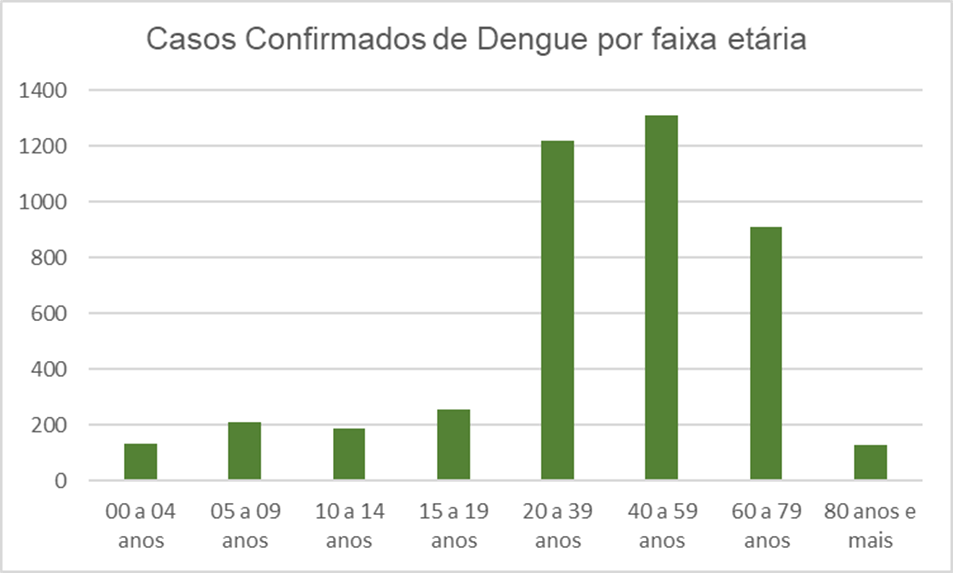
\includegraphics[width=\textwidth]{images/graficos/graf2_dengue.png}
    \fonte{Adaptado de \citeonline{arboviroses}}
\end{grafico}

\section{REVISÃO DE TECNOLOGIAS EXISTENTES}

Após algumas pesquisas realizadas sobre tecnologias já existentes que atendem ao tema apontamos como principais a plataforma E-Ouve e o Cidadera.

O E-Ouve é uma plataforma web e aplicativo mobile utilizada em cidades de diversos estados brasileiros, trata-se de um sistema de ouvidoria para realizar solicitações sobre assuntos variados, cada cidade tem liberdade para selecionar que áreas deseja filtrar e receber denúncias dos munícipes. A plataforma da cidade de Itu recebe problemas referentes Administração/RH, Serviços Urbanos, Podas e Buracos, problemas referentes a CIS (Companhia Ituana de Saneamento), Educação, Obras/Iluminação entre outros.

\begin{figure}[H]
    \centering
    \caption{\label{fig2_eouve}Algumas das áreas atendidas pela cidade de Itu na plataforma E-Ouve}
    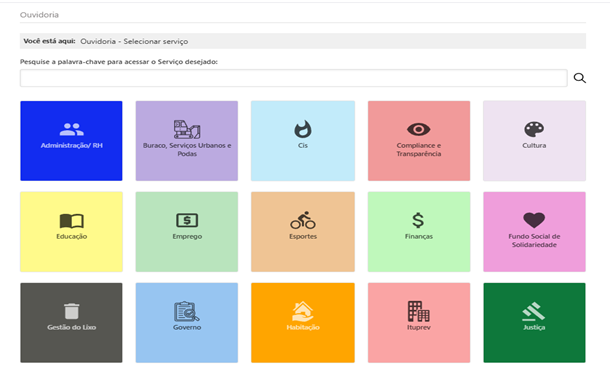
\includegraphics[scale=1.0]{images/figuras/fig2_eouve.png}
    \fonte{\citeonline{eouve}}
\end{figure}

Por se tratar de uma plataforma excessivamente carregada de funcionalidades, ela acaba não tendo o foco principal de receber problemas de fato. Além disso não é amplamente conhecida pela população.

A outra plataforma que podemos citar com conceito similar ao nossa é o Cidadera, desenvolvido em 2013 por alunos do Instituto de Ciências, Matemática e de Computação (ICMC) da Universidade de São Paulo (USP) e alunos da Universidade Federal de São Carlos (UFSCAR). De acordo com um blog publicado na plataforma da USP (2013): “a plataforma é destinada ao mapeamento colaborativo de problemas urbanos, tais como buracos nas ruas, entulho, mato alto e vazamento de água”\cite{app_usp}. O aplicativo não está mais disponível e a plataforma web existente encontra-se com informações sem relação à proposta inicial. 

\begin{figure}[H]
    \centering
    \caption{\label{fig3_cidadera}Plataforma Web do Cidadera}
    
\includegraphics[scale=1.0]{images/figuras/fig3_cidadera.png}
    \fonte{\citeonline{cidadera}. Nota: site atualmente descontinuado.}
\end{figure}

Dadas as tecnologias depreciadas já existentes, revela-se a importância da criação de uma atualizada e com foco específico em reportar os problemas da cidade de Itu.
